\documentclass[twoside]{book}

% Packages required by doxygen
\usepackage{fixltx2e}
\usepackage{calc}
\usepackage{doxygen}
\usepackage[export]{adjustbox} % also loads graphicx
\usepackage{graphicx}
\usepackage[utf8]{inputenc}
\usepackage{makeidx}
\usepackage{multicol}
\usepackage{multirow}
\PassOptionsToPackage{warn}{textcomp}
\usepackage{textcomp}
\usepackage[nointegrals]{wasysym}
\usepackage[table]{xcolor}

% Font selection
\usepackage[T1]{fontenc}
\usepackage[scaled=.90]{helvet}
\usepackage{courier}
\usepackage{amssymb}
\usepackage{sectsty}
\renewcommand{\familydefault}{\sfdefault}
\allsectionsfont{%
  \fontseries{bc}\selectfont%
  \color{darkgray}%
}
\renewcommand{\DoxyLabelFont}{%
  \fontseries{bc}\selectfont%
  \color{darkgray}%
}
\newcommand{\+}{\discretionary{\mbox{\scriptsize$\hookleftarrow$}}{}{}}

% Page & text layout
\usepackage{geometry}
\geometry{%
  a4paper,%
  top=2.5cm,%
  bottom=2.5cm,%
  left=2.5cm,%
  right=2.5cm%
}
\tolerance=750
\hfuzz=15pt
\hbadness=750
\setlength{\emergencystretch}{15pt}
\setlength{\parindent}{0cm}
\setlength{\parskip}{3ex plus 2ex minus 2ex}
\makeatletter
\renewcommand{\paragraph}{%
  \@startsection{paragraph}{4}{0ex}{-1.0ex}{1.0ex}{%
    \normalfont\normalsize\bfseries\SS@parafont%
  }%
}
\renewcommand{\subparagraph}{%
  \@startsection{subparagraph}{5}{0ex}{-1.0ex}{1.0ex}{%
    \normalfont\normalsize\bfseries\SS@subparafont%
  }%
}
\makeatother

% Headers & footers
\usepackage{fancyhdr}
\pagestyle{fancyplain}
\fancyhead[LE]{\fancyplain{}{\bfseries\thepage}}
\fancyhead[CE]{\fancyplain{}{}}
\fancyhead[RE]{\fancyplain{}{\bfseries\leftmark}}
\fancyhead[LO]{\fancyplain{}{\bfseries\rightmark}}
\fancyhead[CO]{\fancyplain{}{}}
\fancyhead[RO]{\fancyplain{}{\bfseries\thepage}}
\fancyfoot[LE]{\fancyplain{}{}}
\fancyfoot[CE]{\fancyplain{}{}}
\fancyfoot[RE]{\fancyplain{}{\bfseries\scriptsize Generated by Doxygen }}
\fancyfoot[LO]{\fancyplain{}{\bfseries\scriptsize Generated by Doxygen }}
\fancyfoot[CO]{\fancyplain{}{}}
\fancyfoot[RO]{\fancyplain{}{}}
\renewcommand{\footrulewidth}{0.4pt}
\renewcommand{\chaptermark}[1]{%
  \markboth{#1}{}%
}
\renewcommand{\sectionmark}[1]{%
  \markright{\thesection\ #1}%
}

% Indices & bibliography
\usepackage{natbib}
\usepackage[titles]{tocloft}
\setcounter{tocdepth}{3}
\setcounter{secnumdepth}{5}
\makeindex

% Hyperlinks (required, but should be loaded last)
\usepackage{ifpdf}
\ifpdf
  \usepackage[pdftex,pagebackref=true]{hyperref}
\else
  \usepackage[ps2pdf,pagebackref=true]{hyperref}
\fi
\hypersetup{%
  colorlinks=true,%
  linkcolor=blue,%
  citecolor=blue,%
  unicode%
}

% Custom commands
\newcommand{\clearemptydoublepage}{%
  \newpage{\pagestyle{empty}\cleardoublepage}%
}

\usepackage{caption}
\captionsetup{labelsep=space,justification=centering,font={bf},singlelinecheck=off,skip=4pt,position=top}

%===== C O N T E N T S =====

\begin{document}

% Titlepage & ToC
\hypersetup{pageanchor=false,
             bookmarksnumbered=true,
             pdfencoding=unicode
            }
\pagenumbering{roman}
\begin{titlepage}
\vspace*{7cm}
\begin{center}%
{\Large psys18 wave equation \\[1ex]\large 1 }\\
\vspace*{1cm}
{\large Generated by Doxygen 1.8.11}\\
\end{center}
\end{titlepage}
\clearemptydoublepage
\tableofcontents
\clearemptydoublepage
\pagenumbering{arabic}
\hypersetup{pageanchor=true}

%--- Begin generated contents ---
\chapter{es\+Ist\+Eine\+W\+E\+L\+LE}
\label{md_README}
\hypertarget{md_README}{}
\input{md_README}
\chapter{File Index}
\section{File List}
Here is a list of all documented files with brief descriptions\+:\begin{DoxyCompactList}
\item\contentsline{section}{\hyperlink{core_8c}{core.\+c} \\*This file contains the main calculation logic for the wave }{\pageref{core_8c}}{}
\item\contentsline{section}{\hyperlink{core_8h}{core.\+h} \\*Main calculation logic for the wave }{\pageref{core_8h}}{}
\item\contentsline{section}{\hyperlink{myWave_8c}{my\+Wave.\+c} \\*This file contains the main program }{\pageref{myWave_8c}}{}
\item\contentsline{section}{\hyperlink{myWave_8h}{my\+Wave.\+h} \\*Main program }{\pageref{myWave_8h}}{}
\end{DoxyCompactList}

\chapter{File Documentation}
\hypertarget{core_8c}{}\section{core.\+c File Reference}
\label{core_8c}\index{core.\+c@{core.\+c}}


This file contains the main calculation logic for the wave.  


{\ttfamily \#include $<$omp.\+h$>$}\\*
{\ttfamily \#include \char`\"{}core.\+h\char`\"{}}\\*
Include dependency graph for core.\+c\+:
\nopagebreak
\begin{figure}[H]
\begin{center}
\leavevmode
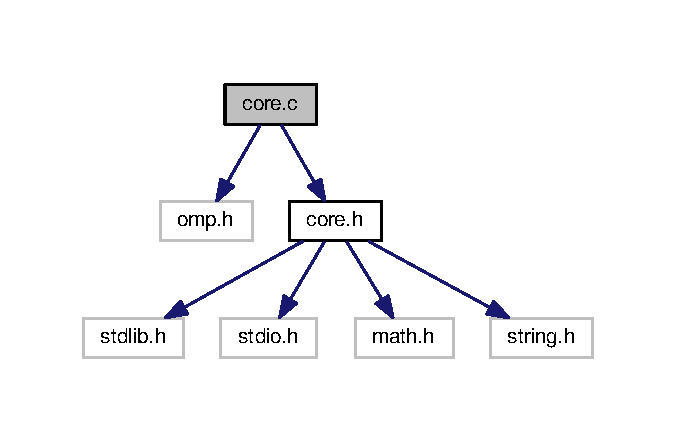
\includegraphics[width=325pt]{core_8c__incl}
\end{center}
\end{figure}
\subsection*{Macros}
\begin{DoxyCompactItemize}
\item 
\#define {\bfseries U\+S\+E\+\_\+\+O\+P\+E\+N\+MP}\hypertarget{core_8c_a01df339826abe970836832ae79e5f894}{}\label{core_8c_a01df339826abe970836832ae79e5f894}

\item 
\#define {\bfseries M\+A\+X\+\_\+\+P\+O\+I\+N\+TS}~10000000\hypertarget{core_8c_a3b8cb7c2cda80c18f333c00601c6905b}{}\label{core_8c_a3b8cb7c2cda80c18f333c00601c6905b}

\item 
\#define {\bfseries M\+A\+X\+\_\+\+L\+A\+M\+B\+DA}~0.\+1\hypertarget{core_8c_a9a3c39851db57d96a225d39850fc20ed}{}\label{core_8c_a9a3c39851db57d96a225d39850fc20ed}

\item 
\#define {\bfseries D\+E\+F\+A\+U\+L\+T\+\_\+\+S\+E\+T\+T\+I\+N\+G\+S\+\_\+\+F\+I\+L\+E\+\_\+\+P\+A\+TH}~\char`\"{}settings.\+txt\char`\"{}\hypertarget{core_8c_ad1f91299f901fda48e4ab3663fcd17e7}{}\label{core_8c_ad1f91299f901fda48e4ab3663fcd17e7}

\end{DoxyCompactItemize}
\subsection*{Functions}
\begin{DoxyCompactItemize}
\item 
double \hyperlink{core_8c_a028b01d036818e96559754619c42d016}{wave\+Init\+Func} (double x)
\item 
void \hyperlink{core_8c_a820d59cad514afd728ba0a96fd29e0bf}{output\+Help\+Message} ()
\item 
void \hyperlink{core_8c_a7ee68549bc08a739d0ef1f9940df0e87}{get\+From\+Settings\+File} (char $\ast$config\+Path)
\item 
void \hyperlink{core_8c_aa5d12f857568f87f84d47706cde89499}{get\+From\+Cmd\+Line} (int nargc, char $\ast$$\ast$argv)
\item 
void \hyperlink{core_8c_a669091cfd4f03bc6a634eb21ed14c496}{check\+Params} ()
\item 
void \hyperlink{core_8c_ac0481d35a5bb56dae20d48123db635fb}{get\+User\+Input\+Or\+Config} (int numberofargc, char $\ast$$\ast$argv)
\item 
void \hyperlink{core_8c_acf4091d39662af3ee96a2666189a0d25}{init\+Wave\+Conditions} ()
\item 
void \hyperlink{core_8c_a42ed0a429bc4ad03ce55d79ce90e2cbf}{simulate\+One\+Time\+Step} (int holdflag)
\item 
void \hyperlink{core_8c_a57fde30c38e9cd0270fe7b03f87d4000}{simulate\+Number\+Of\+Time\+Steps} ()
\item 
void \hyperlink{core_8c_ae9df782277427a2c9e71cee192fe66cf}{finalize\+Wave} ()
\item 
void \hyperlink{core_8c_aebc67ff9f96f58d16c1297807fa6adc6}{reset\+Wave} ()
\item 
void \hyperlink{core_8c_ab2cf5629d024cc5e0826640ae5239000}{output\+New} ()
\item 
double $\ast$ \hyperlink{core_8c_a08b92a703191cfac34519bf26fcfd158}{get\+Step} ()
\item 
int \hyperlink{core_8c_ae9ecf3107ce69567cce1b0d64e7fad22}{get\+N\+P\+O\+I\+N\+TS} ()
\item 
int \hyperlink{core_8c_a7be70a3f8f027affff9e3e226567c551}{get\+T\+P\+O\+I\+N\+TS} ()
\item 
double \hyperlink{core_8c_a1de827e29b2f3bc5c16d330a7c7e9add}{get\+L\+A\+M\+B\+DA} ()
\item 
int \hyperlink{core_8c_a042969b182b78a4ccb8c84636065e5e2}{use\+G\+UI} ()
\end{DoxyCompactItemize}
\subsection*{Variables}
\begin{DoxyCompactItemize}
\item 
const double {\bfseries PI} = 3.\+14159265359\hypertarget{core_8c_a952eac791b596a61bba0a133a3bb439f}{}\label{core_8c_a952eac791b596a61bba0a133a3bb439f}

\item 
int {\bfseries periods}\hypertarget{core_8c_a37d4821bb370cc7c0aeb110809a8a524}{}\label{core_8c_a37d4821bb370cc7c0aeb110809a8a524}

\item 
int {\bfseries amplitude}\hypertarget{core_8c_ad07f93f796ba0af60659c528f7611d4a}{}\label{core_8c_ad07f93f796ba0af60659c528f7611d4a}

\item 
double $\ast$ {\bfseries previous\+Step}\hypertarget{core_8c_aacc30507897378d335eaf79e2d9bc61f}{}\label{core_8c_aacc30507897378d335eaf79e2d9bc61f}

\item 
double $\ast$ {\bfseries current\+Step}\hypertarget{core_8c_a1b3d58342fab0051d558834fabf4b21c}{}\label{core_8c_a1b3d58342fab0051d558834fabf4b21c}

\item 
double $\ast$ {\bfseries next\+Step}\hypertarget{core_8c_a280b656f6f6299a87f1c2193c6fa9267}{}\label{core_8c_a280b656f6f6299a87f1c2193c6fa9267}

\item 
int {\bfseries use\+Gui}\hypertarget{core_8c_a1c9515e11339bc83c87ecfb9dc256b6e}{}\label{core_8c_a1c9515e11339bc83c87ecfb9dc256b6e}

\item 
int {\bfseries printvalues}\hypertarget{core_8c_a743ba990c374dca69ff40a943c659a02}{}\label{core_8c_a743ba990c374dca69ff40a943c659a02}

\item 
int {\bfseries N\+P\+O\+I\+N\+TS}\hypertarget{core_8c_a962b0165b26063be2be3f5e8d9fbcccb}{}\label{core_8c_a962b0165b26063be2be3f5e8d9fbcccb}

\item 
int {\bfseries T\+P\+O\+I\+N\+TS}\hypertarget{core_8c_a48d31056ae3689349eac465857975b54}{}\label{core_8c_a48d31056ae3689349eac465857975b54}

\item 
double {\bfseries D\+E\+L\+T\+A\+\_\+X}\hypertarget{core_8c_a0bfd22b1593e0532383f02386dce590c}{}\label{core_8c_a0bfd22b1593e0532383f02386dce590c}

\item 
double {\bfseries lambda}\hypertarget{core_8c_a3db359547eed8cfd48ca821d95f577af}{}\label{core_8c_a3db359547eed8cfd48ca821d95f577af}

\item 
const double {\bfseries D\+E\+L\+T\+A\+\_\+T} = 1.\+0\hypertarget{core_8c_a187b17b96f16d81cd6a62fb88e0db758}{}\label{core_8c_a187b17b96f16d81cd6a62fb88e0db758}

\item 
int {\bfseries L}\hypertarget{core_8c_a61b43f3326e96036caf1c76875b794cc}{}\label{core_8c_a61b43f3326e96036caf1c76875b794cc}

\item 
double {\bfseries C}\hypertarget{core_8c_a8987032f6f7d7cfaa0ff4e2a62ae08fe}{}\label{core_8c_a8987032f6f7d7cfaa0ff4e2a62ae08fe}

\item 
double {\bfseries C\+\_\+\+S\+Q\+U\+A\+R\+ED}\hypertarget{core_8c_a25f82e8fe009d6699f60996e569900a0}{}\label{core_8c_a25f82e8fe009d6699f60996e569900a0}

\item 
double {\bfseries S\+P\+E\+ED}\hypertarget{core_8c_a93dc260b1444c685c7dc08a9cb3dc9c5}{}\label{core_8c_a93dc260b1444c685c7dc08a9cb3dc9c5}

\end{DoxyCompactItemize}


\subsection{Detailed Description}
This file contains the main calculation logic for the wave. 

Implements the main calculation logic for the wave

\begin{DoxyAuthor}{Author}
Chris Rebbelin s0548921 
\end{DoxyAuthor}
\begin{DoxyDate}{Date}
2018-\/07-\/01 
\end{DoxyDate}


\subsection{Function Documentation}
\index{core.\+c@{core.\+c}!check\+Params@{check\+Params}}
\index{check\+Params@{check\+Params}!core.\+c@{core.\+c}}
\subsubsection[{\texorpdfstring{check\+Params()}{checkParams()}}]{\setlength{\rightskip}{0pt plus 5cm}void check\+Params (
\begin{DoxyParamCaption}
\item[{void}]{}
\end{DoxyParamCaption}
)}\hypertarget{core_8c_a669091cfd4f03bc6a634eb21ed14c496}{}\label{core_8c_a669091cfd4f03bc6a634eb21ed14c496}
Checks all parameters for validity \index{core.\+c@{core.\+c}!finalize\+Wave@{finalize\+Wave}}
\index{finalize\+Wave@{finalize\+Wave}!core.\+c@{core.\+c}}
\subsubsection[{\texorpdfstring{finalize\+Wave()}{finalizeWave()}}]{\setlength{\rightskip}{0pt plus 5cm}void finalize\+Wave (
\begin{DoxyParamCaption}
\item[{void}]{}
\end{DoxyParamCaption}
)}\hypertarget{core_8c_ae9df782277427a2c9e71cee192fe66cf}{}\label{core_8c_ae9df782277427a2c9e71cee192fe66cf}
Frees the memory from the time step arrays \index{core.\+c@{core.\+c}!get\+From\+Cmd\+Line@{get\+From\+Cmd\+Line}}
\index{get\+From\+Cmd\+Line@{get\+From\+Cmd\+Line}!core.\+c@{core.\+c}}
\subsubsection[{\texorpdfstring{get\+From\+Cmd\+Line(int nargc, char $\ast$$\ast$argv)}{getFromCmdLine(int nargc, char **argv)}}]{\setlength{\rightskip}{0pt plus 5cm}void get\+From\+Cmd\+Line (
\begin{DoxyParamCaption}
\item[{int}]{nargc, }
\item[{char $\ast$$\ast$}]{argv}
\end{DoxyParamCaption}
)}\hypertarget{core_8c_aa5d12f857568f87f84d47706cde89499}{}\label{core_8c_aa5d12f857568f87f84d47706cde89499}
Parses the settings from command line


\begin{DoxyParams}{Parameters}
{\em nargc} & argument count of the program \\
\hline
{\em argv} & arguments of the program \\
\hline
\end{DoxyParams}
\index{core.\+c@{core.\+c}!get\+From\+Settings\+File@{get\+From\+Settings\+File}}
\index{get\+From\+Settings\+File@{get\+From\+Settings\+File}!core.\+c@{core.\+c}}
\subsubsection[{\texorpdfstring{get\+From\+Settings\+File(char $\ast$config\+Path)}{getFromSettingsFile(char *configPath)}}]{\setlength{\rightskip}{0pt plus 5cm}void get\+From\+Settings\+File (
\begin{DoxyParamCaption}
\item[{char $\ast$}]{config\+Path}
\end{DoxyParamCaption}
)}\hypertarget{core_8c_a7ee68549bc08a739d0ef1f9940df0e87}{}\label{core_8c_a7ee68549bc08a739d0ef1f9940df0e87}
Reads the settings from file specified by a given file path


\begin{DoxyParams}{Parameters}
{\em config\+Path} & Path to a settings file \\
\hline
\end{DoxyParams}
\index{core.\+c@{core.\+c}!get\+L\+A\+M\+B\+DA@{get\+L\+A\+M\+B\+DA}}
\index{get\+L\+A\+M\+B\+DA@{get\+L\+A\+M\+B\+DA}!core.\+c@{core.\+c}}
\subsubsection[{\texorpdfstring{get\+L\+A\+M\+B\+D\+A()}{getLAMBDA()}}]{\setlength{\rightskip}{0pt plus 5cm}double get\+L\+A\+M\+B\+DA (
\begin{DoxyParamCaption}
\item[{void}]{}
\end{DoxyParamCaption}
)}\hypertarget{core_8c_a1de827e29b2f3bc5c16d330a7c7e9add}{}\label{core_8c_a1de827e29b2f3bc5c16d330a7c7e9add}
Returns the dampening factor lambda.

\begin{DoxyReturn}{Returns}
The dampening factor of the wave 
\end{DoxyReturn}
\index{core.\+c@{core.\+c}!get\+N\+P\+O\+I\+N\+TS@{get\+N\+P\+O\+I\+N\+TS}}
\index{get\+N\+P\+O\+I\+N\+TS@{get\+N\+P\+O\+I\+N\+TS}!core.\+c@{core.\+c}}
\subsubsection[{\texorpdfstring{get\+N\+P\+O\+I\+N\+T\+S()}{getNPOINTS()}}]{\setlength{\rightskip}{0pt plus 5cm}int get\+N\+P\+O\+I\+N\+TS (
\begin{DoxyParamCaption}
\item[{void}]{}
\end{DoxyParamCaption}
)}\hypertarget{core_8c_ae9ecf3107ce69567cce1b0d64e7fad22}{}\label{core_8c_ae9ecf3107ce69567cce1b0d64e7fad22}
Returns the number of discrete points of the wave.

\begin{DoxyReturn}{Returns}
The number of discrete points of the wave 
\end{DoxyReturn}
\index{core.\+c@{core.\+c}!get\+Step@{get\+Step}}
\index{get\+Step@{get\+Step}!core.\+c@{core.\+c}}
\subsubsection[{\texorpdfstring{get\+Step()}{getStep()}}]{\setlength{\rightskip}{0pt plus 5cm}double$\ast$ get\+Step (
\begin{DoxyParamCaption}
\item[{void}]{}
\end{DoxyParamCaption}
)}\hypertarget{core_8c_a08b92a703191cfac34519bf26fcfd158}{}\label{core_8c_a08b92a703191cfac34519bf26fcfd158}
Returns the current state of the wave values.

\begin{DoxyReturn}{Returns}
A pointer to array of the current values 
\end{DoxyReturn}
\index{core.\+c@{core.\+c}!get\+T\+P\+O\+I\+N\+TS@{get\+T\+P\+O\+I\+N\+TS}}
\index{get\+T\+P\+O\+I\+N\+TS@{get\+T\+P\+O\+I\+N\+TS}!core.\+c@{core.\+c}}
\subsubsection[{\texorpdfstring{get\+T\+P\+O\+I\+N\+T\+S()}{getTPOINTS()}}]{\setlength{\rightskip}{0pt plus 5cm}int get\+T\+P\+O\+I\+N\+TS (
\begin{DoxyParamCaption}
\item[{void}]{}
\end{DoxyParamCaption}
)}\hypertarget{core_8c_a7be70a3f8f027affff9e3e226567c551}{}\label{core_8c_a7be70a3f8f027affff9e3e226567c551}
Returns the number of time steps (can be 0 for loop).

\begin{DoxyReturn}{Returns}
The number of time steps 
\end{DoxyReturn}
\index{core.\+c@{core.\+c}!get\+User\+Input\+Or\+Config@{get\+User\+Input\+Or\+Config}}
\index{get\+User\+Input\+Or\+Config@{get\+User\+Input\+Or\+Config}!core.\+c@{core.\+c}}
\subsubsection[{\texorpdfstring{get\+User\+Input\+Or\+Config(int numberofargc, char $\ast$$\ast$argv)}{getUserInputOrConfig(int numberofargc, char **argv)}}]{\setlength{\rightskip}{0pt plus 5cm}void get\+User\+Input\+Or\+Config (
\begin{DoxyParamCaption}
\item[{int}]{numberofargc, }
\item[{char $\ast$$\ast$}]{argv}
\end{DoxyParamCaption}
)}\hypertarget{core_8c_ac0481d35a5bb56dae20d48123db635fb}{}\label{core_8c_ac0481d35a5bb56dae20d48123db635fb}
Reads the given cmd arguments


\begin{DoxyParams}{Parameters}
{\em numberofargc} & argument count of the program \\
\hline
{\em argv} & arguments of the program \\
\hline
\end{DoxyParams}
\index{core.\+c@{core.\+c}!init\+Wave\+Conditions@{init\+Wave\+Conditions}}
\index{init\+Wave\+Conditions@{init\+Wave\+Conditions}!core.\+c@{core.\+c}}
\subsubsection[{\texorpdfstring{init\+Wave\+Conditions()}{initWaveConditions()}}]{\setlength{\rightskip}{0pt plus 5cm}void init\+Wave\+Conditions (
\begin{DoxyParamCaption}
\item[{void}]{}
\end{DoxyParamCaption}
)}\hypertarget{core_8c_acf4091d39662af3ee96a2666189a0d25}{}\label{core_8c_acf4091d39662af3ee96a2666189a0d25}
Allocates the three time step arrays and initializes the first two time steps with the sine curve \index{core.\+c@{core.\+c}!output\+Help\+Message@{output\+Help\+Message}}
\index{output\+Help\+Message@{output\+Help\+Message}!core.\+c@{core.\+c}}
\subsubsection[{\texorpdfstring{output\+Help\+Message()}{outputHelpMessage()}}]{\setlength{\rightskip}{0pt plus 5cm}void output\+Help\+Message (
\begin{DoxyParamCaption}
\item[{void}]{}
\end{DoxyParamCaption}
)}\hypertarget{core_8c_a820d59cad514afd728ba0a96fd29e0bf}{}\label{core_8c_a820d59cad514afd728ba0a96fd29e0bf}
Outputs a help message for the user \index{core.\+c@{core.\+c}!output\+New@{output\+New}}
\index{output\+New@{output\+New}!core.\+c@{core.\+c}}
\subsubsection[{\texorpdfstring{output\+New()}{outputNew()}}]{\setlength{\rightskip}{0pt plus 5cm}void output\+New (
\begin{DoxyParamCaption}
\item[{void}]{}
\end{DoxyParamCaption}
)}\hypertarget{core_8c_ab2cf5629d024cc5e0826640ae5239000}{}\label{core_8c_ab2cf5629d024cc5e0826640ae5239000}
Prints the new time step array values to console \index{core.\+c@{core.\+c}!reset\+Wave@{reset\+Wave}}
\index{reset\+Wave@{reset\+Wave}!core.\+c@{core.\+c}}
\subsubsection[{\texorpdfstring{reset\+Wave()}{resetWave()}}]{\setlength{\rightskip}{0pt plus 5cm}void reset\+Wave (
\begin{DoxyParamCaption}
\item[{void}]{}
\end{DoxyParamCaption}
)}\hypertarget{core_8c_aebc67ff9f96f58d16c1297807fa6adc6}{}\label{core_8c_aebc67ff9f96f58d16c1297807fa6adc6}
Resets the time step arrays to the inital sine wave. \index{core.\+c@{core.\+c}!simulate\+Number\+Of\+Time\+Steps@{simulate\+Number\+Of\+Time\+Steps}}
\index{simulate\+Number\+Of\+Time\+Steps@{simulate\+Number\+Of\+Time\+Steps}!core.\+c@{core.\+c}}
\subsubsection[{\texorpdfstring{simulate\+Number\+Of\+Time\+Steps()}{simulateNumberOfTimeSteps()}}]{\setlength{\rightskip}{0pt plus 5cm}void simulate\+Number\+Of\+Time\+Steps (
\begin{DoxyParamCaption}
\item[{void}]{}
\end{DoxyParamCaption}
)}\hypertarget{core_8c_a57fde30c38e9cd0270fe7b03f87d4000}{}\label{core_8c_a57fde30c38e9cd0270fe7b03f87d4000}
Call \hyperlink{core_8h_a42ed0a429bc4ad03ce55d79ce90e2cbf}{simulate\+One\+Time\+Step()} a specified number of times \index{core.\+c@{core.\+c}!simulate\+One\+Time\+Step@{simulate\+One\+Time\+Step}}
\index{simulate\+One\+Time\+Step@{simulate\+One\+Time\+Step}!core.\+c@{core.\+c}}
\subsubsection[{\texorpdfstring{simulate\+One\+Time\+Step(int holdflag)}{simulateOneTimeStep(int holdflag)}}]{\setlength{\rightskip}{0pt plus 5cm}void simulate\+One\+Time\+Step (
\begin{DoxyParamCaption}
\item[{int}]{holdflag}
\end{DoxyParamCaption}
)}\hypertarget{core_8c_a42ed0a429bc4ad03ce55d79ce90e2cbf}{}\label{core_8c_a42ed0a429bc4ad03ce55d79ce90e2cbf}
Simulate one time step with the wave equation \index{core.\+c@{core.\+c}!use\+G\+UI@{use\+G\+UI}}
\index{use\+G\+UI@{use\+G\+UI}!core.\+c@{core.\+c}}
\subsubsection[{\texorpdfstring{use\+G\+U\+I()}{useGUI()}}]{\setlength{\rightskip}{0pt plus 5cm}int use\+G\+UI (
\begin{DoxyParamCaption}
\item[{void}]{}
\end{DoxyParamCaption}
)}\hypertarget{core_8c_a042969b182b78a4ccb8c84636065e5e2}{}\label{core_8c_a042969b182b78a4ccb8c84636065e5e2}
Returns the current state of the show\+Gui flag.

\begin{DoxyReturn}{Returns}
Whether to show the wave or not 
\end{DoxyReturn}
\index{core.\+c@{core.\+c}!wave\+Init\+Func@{wave\+Init\+Func}}
\index{wave\+Init\+Func@{wave\+Init\+Func}!core.\+c@{core.\+c}}
\subsubsection[{\texorpdfstring{wave\+Init\+Func(double x)}{waveInitFunc(double x)}}]{\setlength{\rightskip}{0pt plus 5cm}double wave\+Init\+Func (
\begin{DoxyParamCaption}
\item[{double}]{x}
\end{DoxyParamCaption}
)}\hypertarget{core_8c_a028b01d036818e96559754619c42d016}{}\label{core_8c_a028b01d036818e96559754619c42d016}
Calculates the initial sine wave values


\begin{DoxyParams}{Parameters}
{\em x} & The x value \\
\hline
\end{DoxyParams}
\begin{DoxyReturn}{Returns}
The value of the sine function at x 
\end{DoxyReturn}

\hypertarget{core_8h}{}\section{core.\+h File Reference}
\label{core_8h}\index{core.\+h@{core.\+h}}


contains the main calculation logic for the wave  


{\ttfamily \#include $<$stdlib.\+h$>$}\\*
{\ttfamily \#include $<$stdio.\+h$>$}\\*
{\ttfamily \#include $<$math.\+h$>$}\\*
{\ttfamily \#include $<$string.\+h$>$}\\*
Include dependency graph for core.\+h\+:
\nopagebreak
\begin{figure}[H]
\begin{center}
\leavevmode
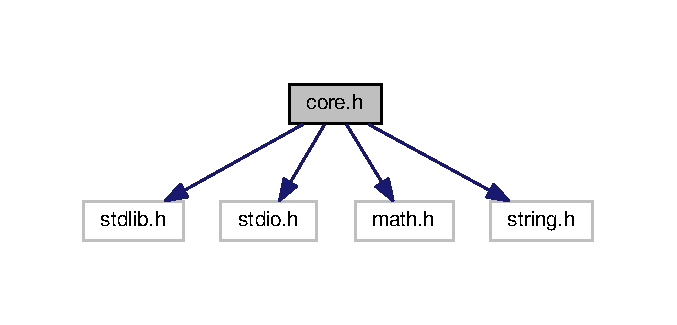
\includegraphics[width=325pt]{core_8h__incl}
\end{center}
\end{figure}
This graph shows which files directly or indirectly include this file\+:
\nopagebreak
\begin{figure}[H]
\begin{center}
\leavevmode
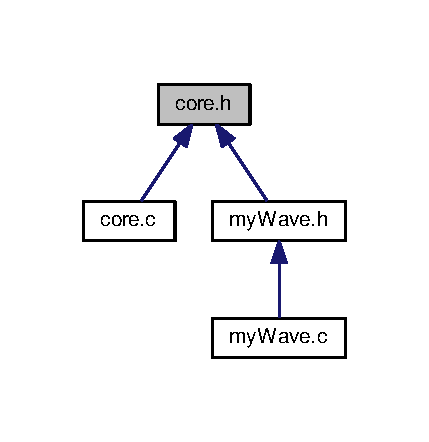
\includegraphics[width=206pt]{core_8h__dep__incl}
\end{center}
\end{figure}
\subsection*{Functions}
\begin{DoxyCompactItemize}
\item 
double \hyperlink{core_8h_a028b01d036818e96559754619c42d016}{wave\+Init\+Func} (double x)
\item 
void \hyperlink{core_8h_a7ee68549bc08a739d0ef1f9940df0e87}{get\+From\+Settings\+File} (char $\ast$config\+Path)
\item 
void \hyperlink{core_8h_aa5d12f857568f87f84d47706cde89499}{get\+From\+Cmd\+Line} (int nargc, char $\ast$$\ast$argv)
\item 
void \hyperlink{core_8h_ac0481d35a5bb56dae20d48123db635fb}{get\+User\+Input\+Or\+Config} (int numberofargc, char $\ast$$\ast$argv)
\item 
void \hyperlink{core_8h_a059448ca6fd54fb2787a667e80369699}{output\+Help\+Message} (void)
\item 
void \hyperlink{core_8h_a7715c03c8f55a9a74822ddf5d2189161}{check\+Params} (void)
\item 
void \hyperlink{core_8h_af4789aa9b6fab181913c6594f2605c85}{init\+Wave\+Conditions} (void)
\item 
void \hyperlink{core_8h_a42ed0a429bc4ad03ce55d79ce90e2cbf}{simulate\+One\+Time\+Step} (int holdflag)
\item 
void \hyperlink{core_8h_a1f3551acd5b063b3ecd74f92c1ca0527}{simulate\+Number\+Of\+Time\+Steps} (void)
\item 
void \hyperlink{core_8h_af51cb3b7f9d918bbadc733a2312edb21}{finalize\+Wave} (void)
\item 
void \hyperlink{core_8h_afbdbf53e941a7bba345414a84c8214ae}{reset\+Wave} (void)
\item 
void \hyperlink{core_8h_a0331cd95eef840f9a1b484ba4cb55ddc}{output\+New} (void)
\item 
double $\ast$ \hyperlink{core_8h_a7e32fe3a1ddcaaec77da0b618edc7eb9}{get\+Step} (void)
\item 
int \hyperlink{core_8h_a2ad79e29e44ccf1dd678dd8470f7051d}{get\+N\+P\+O\+I\+N\+TS} (void)
\item 
int \hyperlink{core_8h_ac739b4bf6bc3b269f5665208fd558cb0}{get\+T\+P\+O\+I\+N\+TS} (void)
\item 
double \hyperlink{core_8h_a90b1f87958a12d9cb7f7418f58cd2e90}{get\+L\+A\+M\+B\+DA} (void)
\item 
int \hyperlink{core_8h_a03455a66467ff59f893aa0bbf96bccdf}{use\+G\+UI} (void)
\end{DoxyCompactItemize}


\subsection{Detailed Description}
contains the main calculation logic for the wave 

\begin{DoxyAuthor}{Author}
Chris Rebbelin s0548921 
\end{DoxyAuthor}
\begin{DoxyDate}{Date}
2018-\/07-\/01 
\end{DoxyDate}


\subsection{Function Documentation}
\index{core.\+h@{core.\+h}!check\+Params@{check\+Params}}
\index{check\+Params@{check\+Params}!core.\+h@{core.\+h}}
\subsubsection[{\texorpdfstring{check\+Params(void)}{checkParams(void)}}]{\setlength{\rightskip}{0pt plus 5cm}void check\+Params (
\begin{DoxyParamCaption}
\item[{void}]{}
\end{DoxyParamCaption}
)}\hypertarget{core_8h_a7715c03c8f55a9a74822ddf5d2189161}{}\label{core_8h_a7715c03c8f55a9a74822ddf5d2189161}
Checks all parameters for validity \index{core.\+h@{core.\+h}!finalize\+Wave@{finalize\+Wave}}
\index{finalize\+Wave@{finalize\+Wave}!core.\+h@{core.\+h}}
\subsubsection[{\texorpdfstring{finalize\+Wave(void)}{finalizeWave(void)}}]{\setlength{\rightskip}{0pt plus 5cm}void finalize\+Wave (
\begin{DoxyParamCaption}
\item[{void}]{}
\end{DoxyParamCaption}
)}\hypertarget{core_8h_af51cb3b7f9d918bbadc733a2312edb21}{}\label{core_8h_af51cb3b7f9d918bbadc733a2312edb21}
Frees the memory from the time step arrays \index{core.\+h@{core.\+h}!get\+From\+Cmd\+Line@{get\+From\+Cmd\+Line}}
\index{get\+From\+Cmd\+Line@{get\+From\+Cmd\+Line}!core.\+h@{core.\+h}}
\subsubsection[{\texorpdfstring{get\+From\+Cmd\+Line(int nargc, char $\ast$$\ast$argv)}{getFromCmdLine(int nargc, char **argv)}}]{\setlength{\rightskip}{0pt plus 5cm}void get\+From\+Cmd\+Line (
\begin{DoxyParamCaption}
\item[{int}]{nargc, }
\item[{char $\ast$$\ast$}]{argv}
\end{DoxyParamCaption}
)}\hypertarget{core_8h_aa5d12f857568f87f84d47706cde89499}{}\label{core_8h_aa5d12f857568f87f84d47706cde89499}
Parses the settings from command line


\begin{DoxyParams}{Parameters}
{\em nargc} & argument count of the program \\
\hline
{\em argv} & arguments of the program \\
\hline
\end{DoxyParams}
\index{core.\+h@{core.\+h}!get\+From\+Settings\+File@{get\+From\+Settings\+File}}
\index{get\+From\+Settings\+File@{get\+From\+Settings\+File}!core.\+h@{core.\+h}}
\subsubsection[{\texorpdfstring{get\+From\+Settings\+File(char $\ast$config\+Path)}{getFromSettingsFile(char *configPath)}}]{\setlength{\rightskip}{0pt plus 5cm}void get\+From\+Settings\+File (
\begin{DoxyParamCaption}
\item[{char $\ast$}]{config\+Path}
\end{DoxyParamCaption}
)}\hypertarget{core_8h_a7ee68549bc08a739d0ef1f9940df0e87}{}\label{core_8h_a7ee68549bc08a739d0ef1f9940df0e87}
Reads the settings from file specified by a given file path


\begin{DoxyParams}{Parameters}
{\em config\+Path} & Path to a settings file \\
\hline
\end{DoxyParams}
\index{core.\+h@{core.\+h}!get\+L\+A\+M\+B\+DA@{get\+L\+A\+M\+B\+DA}}
\index{get\+L\+A\+M\+B\+DA@{get\+L\+A\+M\+B\+DA}!core.\+h@{core.\+h}}
\subsubsection[{\texorpdfstring{get\+L\+A\+M\+B\+D\+A(void)}{getLAMBDA(void)}}]{\setlength{\rightskip}{0pt plus 5cm}double get\+L\+A\+M\+B\+DA (
\begin{DoxyParamCaption}
\item[{void}]{}
\end{DoxyParamCaption}
)}\hypertarget{core_8h_a90b1f87958a12d9cb7f7418f58cd2e90}{}\label{core_8h_a90b1f87958a12d9cb7f7418f58cd2e90}
Returns the dampening factor lambda.

\begin{DoxyReturn}{Returns}
The dampening factor of the wave 
\end{DoxyReturn}
\index{core.\+h@{core.\+h}!get\+N\+P\+O\+I\+N\+TS@{get\+N\+P\+O\+I\+N\+TS}}
\index{get\+N\+P\+O\+I\+N\+TS@{get\+N\+P\+O\+I\+N\+TS}!core.\+h@{core.\+h}}
\subsubsection[{\texorpdfstring{get\+N\+P\+O\+I\+N\+T\+S(void)}{getNPOINTS(void)}}]{\setlength{\rightskip}{0pt plus 5cm}int get\+N\+P\+O\+I\+N\+TS (
\begin{DoxyParamCaption}
\item[{void}]{}
\end{DoxyParamCaption}
)}\hypertarget{core_8h_a2ad79e29e44ccf1dd678dd8470f7051d}{}\label{core_8h_a2ad79e29e44ccf1dd678dd8470f7051d}
Returns the number of discrete points of the wave.

\begin{DoxyReturn}{Returns}
The number of discrete points of the wave 
\end{DoxyReturn}
\index{core.\+h@{core.\+h}!get\+Step@{get\+Step}}
\index{get\+Step@{get\+Step}!core.\+h@{core.\+h}}
\subsubsection[{\texorpdfstring{get\+Step(void)}{getStep(void)}}]{\setlength{\rightskip}{0pt plus 5cm}double$\ast$ get\+Step (
\begin{DoxyParamCaption}
\item[{void}]{}
\end{DoxyParamCaption}
)}\hypertarget{core_8h_a7e32fe3a1ddcaaec77da0b618edc7eb9}{}\label{core_8h_a7e32fe3a1ddcaaec77da0b618edc7eb9}
Returns the current state of the wave values.

\begin{DoxyReturn}{Returns}
A pointer to array of the current values 
\end{DoxyReturn}
\index{core.\+h@{core.\+h}!get\+T\+P\+O\+I\+N\+TS@{get\+T\+P\+O\+I\+N\+TS}}
\index{get\+T\+P\+O\+I\+N\+TS@{get\+T\+P\+O\+I\+N\+TS}!core.\+h@{core.\+h}}
\subsubsection[{\texorpdfstring{get\+T\+P\+O\+I\+N\+T\+S(void)}{getTPOINTS(void)}}]{\setlength{\rightskip}{0pt plus 5cm}int get\+T\+P\+O\+I\+N\+TS (
\begin{DoxyParamCaption}
\item[{void}]{}
\end{DoxyParamCaption}
)}\hypertarget{core_8h_ac739b4bf6bc3b269f5665208fd558cb0}{}\label{core_8h_ac739b4bf6bc3b269f5665208fd558cb0}
Returns the number of time steps (can be 0 for loop).

\begin{DoxyReturn}{Returns}
The number of time steps 
\end{DoxyReturn}
\index{core.\+h@{core.\+h}!get\+User\+Input\+Or\+Config@{get\+User\+Input\+Or\+Config}}
\index{get\+User\+Input\+Or\+Config@{get\+User\+Input\+Or\+Config}!core.\+h@{core.\+h}}
\subsubsection[{\texorpdfstring{get\+User\+Input\+Or\+Config(int numberofargc, char $\ast$$\ast$argv)}{getUserInputOrConfig(int numberofargc, char **argv)}}]{\setlength{\rightskip}{0pt plus 5cm}void get\+User\+Input\+Or\+Config (
\begin{DoxyParamCaption}
\item[{int}]{numberofargc, }
\item[{char $\ast$$\ast$}]{argv}
\end{DoxyParamCaption}
)}\hypertarget{core_8h_ac0481d35a5bb56dae20d48123db635fb}{}\label{core_8h_ac0481d35a5bb56dae20d48123db635fb}
Reads the given cmd arguments


\begin{DoxyParams}{Parameters}
{\em numberofargc} & argument count of the program \\
\hline
{\em argv} & arguments of the program \\
\hline
\end{DoxyParams}
\index{core.\+h@{core.\+h}!init\+Wave\+Conditions@{init\+Wave\+Conditions}}
\index{init\+Wave\+Conditions@{init\+Wave\+Conditions}!core.\+h@{core.\+h}}
\subsubsection[{\texorpdfstring{init\+Wave\+Conditions(void)}{initWaveConditions(void)}}]{\setlength{\rightskip}{0pt plus 5cm}void init\+Wave\+Conditions (
\begin{DoxyParamCaption}
\item[{void}]{}
\end{DoxyParamCaption}
)}\hypertarget{core_8h_af4789aa9b6fab181913c6594f2605c85}{}\label{core_8h_af4789aa9b6fab181913c6594f2605c85}
Allocates the three time step arrays and initializes the first two time steps with the sine curve \index{core.\+h@{core.\+h}!output\+Help\+Message@{output\+Help\+Message}}
\index{output\+Help\+Message@{output\+Help\+Message}!core.\+h@{core.\+h}}
\subsubsection[{\texorpdfstring{output\+Help\+Message(void)}{outputHelpMessage(void)}}]{\setlength{\rightskip}{0pt plus 5cm}void output\+Help\+Message (
\begin{DoxyParamCaption}
\item[{void}]{}
\end{DoxyParamCaption}
)}\hypertarget{core_8h_a059448ca6fd54fb2787a667e80369699}{}\label{core_8h_a059448ca6fd54fb2787a667e80369699}
Outputs a help message for the user \index{core.\+h@{core.\+h}!output\+New@{output\+New}}
\index{output\+New@{output\+New}!core.\+h@{core.\+h}}
\subsubsection[{\texorpdfstring{output\+New(void)}{outputNew(void)}}]{\setlength{\rightskip}{0pt plus 5cm}void output\+New (
\begin{DoxyParamCaption}
\item[{void}]{}
\end{DoxyParamCaption}
)}\hypertarget{core_8h_a0331cd95eef840f9a1b484ba4cb55ddc}{}\label{core_8h_a0331cd95eef840f9a1b484ba4cb55ddc}
Prints the new time step array values to console \index{core.\+h@{core.\+h}!reset\+Wave@{reset\+Wave}}
\index{reset\+Wave@{reset\+Wave}!core.\+h@{core.\+h}}
\subsubsection[{\texorpdfstring{reset\+Wave(void)}{resetWave(void)}}]{\setlength{\rightskip}{0pt plus 5cm}void reset\+Wave (
\begin{DoxyParamCaption}
\item[{void}]{}
\end{DoxyParamCaption}
)}\hypertarget{core_8h_afbdbf53e941a7bba345414a84c8214ae}{}\label{core_8h_afbdbf53e941a7bba345414a84c8214ae}
Resets the time step arrays to the inital sine wave. \index{core.\+h@{core.\+h}!simulate\+Number\+Of\+Time\+Steps@{simulate\+Number\+Of\+Time\+Steps}}
\index{simulate\+Number\+Of\+Time\+Steps@{simulate\+Number\+Of\+Time\+Steps}!core.\+h@{core.\+h}}
\subsubsection[{\texorpdfstring{simulate\+Number\+Of\+Time\+Steps(void)}{simulateNumberOfTimeSteps(void)}}]{\setlength{\rightskip}{0pt plus 5cm}void simulate\+Number\+Of\+Time\+Steps (
\begin{DoxyParamCaption}
\item[{void}]{}
\end{DoxyParamCaption}
)}\hypertarget{core_8h_a1f3551acd5b063b3ecd74f92c1ca0527}{}\label{core_8h_a1f3551acd5b063b3ecd74f92c1ca0527}
Call \hyperlink{core_8h_a42ed0a429bc4ad03ce55d79ce90e2cbf}{simulate\+One\+Time\+Step()} a specified number of times \index{core.\+h@{core.\+h}!simulate\+One\+Time\+Step@{simulate\+One\+Time\+Step}}
\index{simulate\+One\+Time\+Step@{simulate\+One\+Time\+Step}!core.\+h@{core.\+h}}
\subsubsection[{\texorpdfstring{simulate\+One\+Time\+Step(int holdflag)}{simulateOneTimeStep(int holdflag)}}]{\setlength{\rightskip}{0pt plus 5cm}void simulate\+One\+Time\+Step (
\begin{DoxyParamCaption}
\item[{int}]{holdflag}
\end{DoxyParamCaption}
)}\hypertarget{core_8h_a42ed0a429bc4ad03ce55d79ce90e2cbf}{}\label{core_8h_a42ed0a429bc4ad03ce55d79ce90e2cbf}
Simulate one time step with the wave equation \index{core.\+h@{core.\+h}!use\+G\+UI@{use\+G\+UI}}
\index{use\+G\+UI@{use\+G\+UI}!core.\+h@{core.\+h}}
\subsubsection[{\texorpdfstring{use\+G\+U\+I(void)}{useGUI(void)}}]{\setlength{\rightskip}{0pt plus 5cm}int use\+G\+UI (
\begin{DoxyParamCaption}
\item[{void}]{}
\end{DoxyParamCaption}
)}\hypertarget{core_8h_a03455a66467ff59f893aa0bbf96bccdf}{}\label{core_8h_a03455a66467ff59f893aa0bbf96bccdf}
Returns the current state of the show\+Gui flag.

\begin{DoxyReturn}{Returns}
Whether to show the wave or not 
\end{DoxyReturn}
\index{core.\+h@{core.\+h}!wave\+Init\+Func@{wave\+Init\+Func}}
\index{wave\+Init\+Func@{wave\+Init\+Func}!core.\+h@{core.\+h}}
\subsubsection[{\texorpdfstring{wave\+Init\+Func(double x)}{waveInitFunc(double x)}}]{\setlength{\rightskip}{0pt plus 5cm}double wave\+Init\+Func (
\begin{DoxyParamCaption}
\item[{double}]{x}
\end{DoxyParamCaption}
)}\hypertarget{core_8h_a028b01d036818e96559754619c42d016}{}\label{core_8h_a028b01d036818e96559754619c42d016}
Calculates the initial sine wave values


\begin{DoxyParams}{Parameters}
{\em x} & The x value \\
\hline
\end{DoxyParams}
\begin{DoxyReturn}{Returns}
The value of the sine function at x 
\end{DoxyReturn}

\hypertarget{myWave_8c}{}\section{my\+Wave.\+c File Reference}
\label{myWave_8c}\index{my\+Wave.\+c@{my\+Wave.\+c}}


This file contains the main program.  


{\ttfamily \#include \char`\"{}my\+Wave.\+h\char`\"{}}\\*
Include dependency graph for my\+Wave.\+c\+:
\nopagebreak
\begin{figure}[H]
\begin{center}
\leavevmode
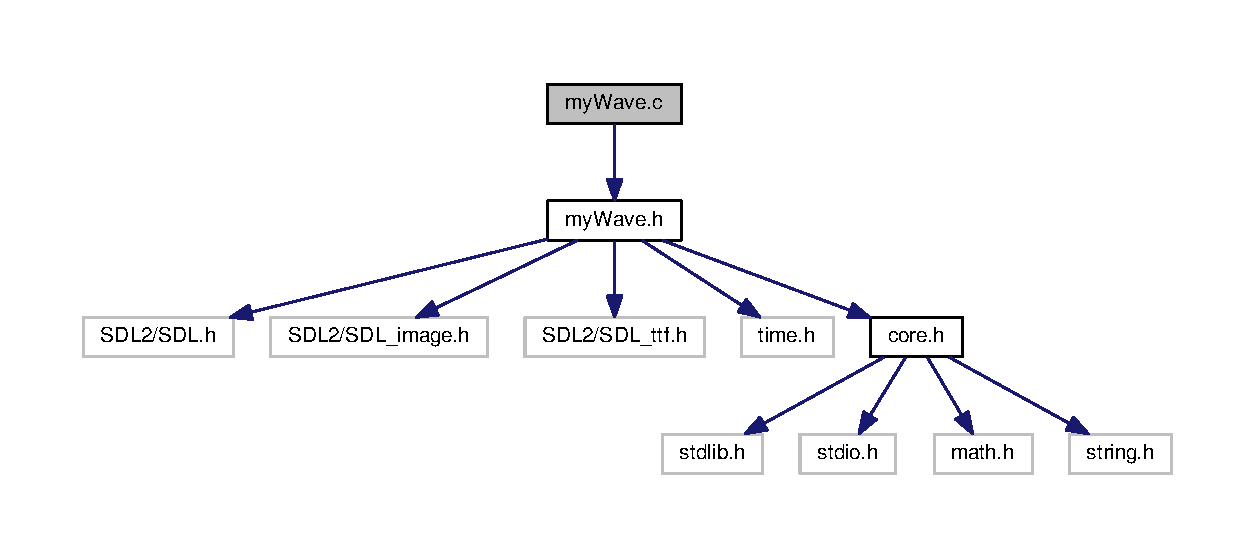
\includegraphics[width=350pt]{myWave_8c__incl}
\end{center}
\end{figure}
\subsection*{Macros}
\begin{DoxyCompactItemize}
\item 
\#define {\bfseries M\+Y\+\_\+\+W\+I\+N\+D\+O\+W\+\_\+\+W\+I\+D\+HT}~1024\hypertarget{myWave_8c_ac2e26d3124b580803153bf9938a692a8}{}\label{myWave_8c_ac2e26d3124b580803153bf9938a692a8}

\item 
\#define {\bfseries M\+Y\+\_\+\+W\+I\+N\+D\+O\+W\+\_\+\+H\+E\+I\+G\+HT}~720\hypertarget{myWave_8c_acaf3b58eaefb27cfbcea880785934dc6}{}\label{myWave_8c_acaf3b58eaefb27cfbcea880785934dc6}

\item 
\#define {\bfseries W\+I\+D\+T\+H\+\_\+\+O\+F\+F\+S\+ET}~20\hypertarget{myWave_8c_a6a6dbe125418de8a9f11943d009ef9ae}{}\label{myWave_8c_a6a6dbe125418de8a9f11943d009ef9ae}

\item 
\#define {\bfseries Y\+\_\+\+A\+X\+I\+S\+\_\+\+L\+E\+N\+G\+TH}~256\hypertarget{myWave_8c_a19f5b38cb67cf6096ad59aa9ecfe7685}{}\label{myWave_8c_a19f5b38cb67cf6096ad59aa9ecfe7685}

\item 
\#define {\bfseries H\+O\+L\+D\+\_\+\+T\+O\+L\+E\+R\+A\+N\+CE}~20\hypertarget{myWave_8c_ab3a3306c90210cba781c3a3f91b07538}{}\label{myWave_8c_ab3a3306c90210cba781c3a3f91b07538}

\end{DoxyCompactItemize}
\subsection*{Functions}
\begin{DoxyCompactItemize}
\item 
void \hyperlink{myWave_8c_ade82befa6e7b024eb4caa3005b74d9ff}{init\+Sdl\+Vars} (S\+D\+L\+\_\+\+Window $\ast$$\ast$win, S\+D\+L\+\_\+\+Renderer $\ast$$\ast$ren, T\+T\+F\+\_\+\+Font $\ast$$\ast$fon)
\item 
void \hyperlink{myWave_8c_a3a48a942f1505a1f3e7178059cbeaea2}{do\+Graphics} ()
\item 
int {\bfseries main} (int argc, char $\ast$$\ast$argv)\hypertarget{myWave_8c_a3c04138a5bfe5d72780bb7e82a18e627}{}\label{myWave_8c_a3c04138a5bfe5d72780bb7e82a18e627}

\end{DoxyCompactItemize}


\subsection{Detailed Description}
This file contains the main program. 

Implements the main program and visualisation to the user

\begin{DoxyAuthor}{Author}
Chris Rebbelin s0548921 
\end{DoxyAuthor}
\begin{DoxyDate}{Date}
2018-\/07-\/01 
\end{DoxyDate}


\subsection{Function Documentation}
\index{my\+Wave.\+c@{my\+Wave.\+c}!do\+Graphics@{do\+Graphics}}
\index{do\+Graphics@{do\+Graphics}!my\+Wave.\+c@{my\+Wave.\+c}}
\subsubsection[{\texorpdfstring{do\+Graphics()}{doGraphics()}}]{\setlength{\rightskip}{0pt plus 5cm}void do\+Graphics (
\begin{DoxyParamCaption}
\item[{void}]{}
\end{DoxyParamCaption}
)}\hypertarget{myWave_8c_a3a48a942f1505a1f3e7178059cbeaea2}{}\label{myWave_8c_a3a48a942f1505a1f3e7178059cbeaea2}
Visualizes the wave equation with the given parameters with the S\+DL library. \index{my\+Wave.\+c@{my\+Wave.\+c}!init\+Sdl\+Vars@{init\+Sdl\+Vars}}
\index{init\+Sdl\+Vars@{init\+Sdl\+Vars}!my\+Wave.\+c@{my\+Wave.\+c}}
\subsubsection[{\texorpdfstring{init\+Sdl\+Vars(\+S\+D\+L\+\_\+\+Window $\ast$$\ast$win, S\+D\+L\+\_\+\+Renderer $\ast$$\ast$ren, T\+T\+F\+\_\+\+Font $\ast$$\ast$fon)}{initSdlVars(SDL_Window **win, SDL_Renderer **ren, TTF_Font **fon)}}]{\setlength{\rightskip}{0pt plus 5cm}void init\+Sdl\+Vars (
\begin{DoxyParamCaption}
\item[{S\+D\+L\+\_\+\+Window $\ast$$\ast$}]{win, }
\item[{S\+D\+L\+\_\+\+Renderer $\ast$$\ast$}]{ren, }
\item[{T\+T\+F\+\_\+\+Font $\ast$$\ast$}]{fon}
\end{DoxyParamCaption}
)}\hypertarget{myWave_8c_ade82befa6e7b024eb4caa3005b74d9ff}{}\label{myWave_8c_ade82befa6e7b024eb4caa3005b74d9ff}
Initializes all needed S\+DL variables.


\begin{DoxyParams}{Parameters}
{\em win} & pointer to the S\+D\+L\+\_\+\+Window \\
\hline
{\em ren} & pointer to the S\+D\+L\+\_\+\+Renderer \\
\hline
{\em fon} & pointer to the T\+T\+F\+\_\+\+Font \\
\hline
\end{DoxyParams}

\hypertarget{myWave_8h}{}\section{my\+Wave.\+h File Reference}
\label{myWave_8h}\index{my\+Wave.\+h@{my\+Wave.\+h}}


contains the main program  


{\ttfamily \#include $<$S\+D\+L2/\+S\+D\+L.\+h$>$}\\*
{\ttfamily \#include $<$S\+D\+L2/\+S\+D\+L\+\_\+image.\+h$>$}\\*
{\ttfamily \#include $<$S\+D\+L2/\+S\+D\+L\+\_\+ttf.\+h$>$}\\*
{\ttfamily \#include $<$time.\+h$>$}\\*
{\ttfamily \#include \char`\"{}core.\+h\char`\"{}}\\*
Include dependency graph for my\+Wave.\+h\+:
\nopagebreak
\begin{figure}[H]
\begin{center}
\leavevmode
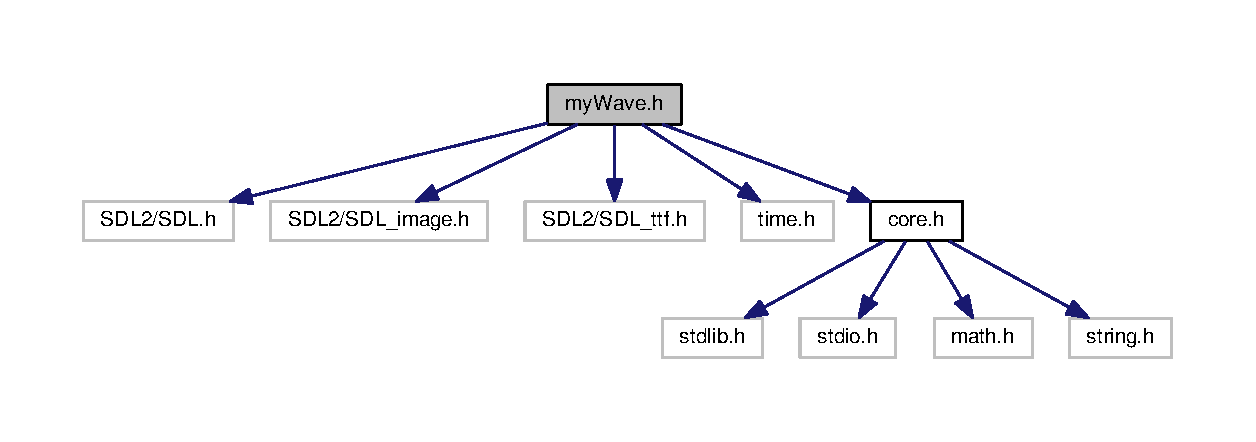
\includegraphics[width=350pt]{myWave_8h__incl}
\end{center}
\end{figure}
This graph shows which files directly or indirectly include this file\+:
\nopagebreak
\begin{figure}[H]
\begin{center}
\leavevmode
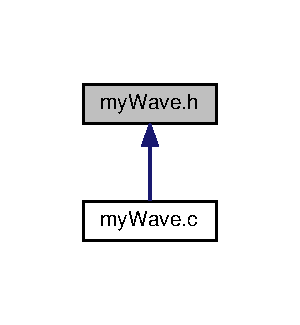
\includegraphics[width=144pt]{myWave_8h__dep__incl}
\end{center}
\end{figure}
\subsection*{Functions}
\begin{DoxyCompactItemize}
\item 
void \hyperlink{myWave_8h_a75fd71424c598545d6f9d1e4e96957be}{do\+Graphics} (void)
\item 
void \hyperlink{myWave_8h_ade82befa6e7b024eb4caa3005b74d9ff}{init\+Sdl\+Vars} (S\+D\+L\+\_\+\+Window $\ast$$\ast$win, S\+D\+L\+\_\+\+Renderer $\ast$$\ast$ren, T\+T\+F\+\_\+\+Font $\ast$$\ast$fon)
\end{DoxyCompactItemize}


\subsection{Detailed Description}
contains the main program 

\begin{DoxyAuthor}{Author}
Chris Rebbelin s0548921 
\end{DoxyAuthor}
\begin{DoxyDate}{Date}
2018-\/07-\/01 
\end{DoxyDate}


\subsection{Function Documentation}
\index{my\+Wave.\+h@{my\+Wave.\+h}!do\+Graphics@{do\+Graphics}}
\index{do\+Graphics@{do\+Graphics}!my\+Wave.\+h@{my\+Wave.\+h}}
\subsubsection[{\texorpdfstring{do\+Graphics(void)}{doGraphics(void)}}]{\setlength{\rightskip}{0pt plus 5cm}void do\+Graphics (
\begin{DoxyParamCaption}
\item[{void}]{}
\end{DoxyParamCaption}
)}\hypertarget{myWave_8h_a75fd71424c598545d6f9d1e4e96957be}{}\label{myWave_8h_a75fd71424c598545d6f9d1e4e96957be}
Visualizes the wave equation with the given parameters with the S\+DL library. \index{my\+Wave.\+h@{my\+Wave.\+h}!init\+Sdl\+Vars@{init\+Sdl\+Vars}}
\index{init\+Sdl\+Vars@{init\+Sdl\+Vars}!my\+Wave.\+h@{my\+Wave.\+h}}
\subsubsection[{\texorpdfstring{init\+Sdl\+Vars(\+S\+D\+L\+\_\+\+Window $\ast$$\ast$win, S\+D\+L\+\_\+\+Renderer $\ast$$\ast$ren, T\+T\+F\+\_\+\+Font $\ast$$\ast$fon)}{initSdlVars(SDL_Window **win, SDL_Renderer **ren, TTF_Font **fon)}}]{\setlength{\rightskip}{0pt plus 5cm}void init\+Sdl\+Vars (
\begin{DoxyParamCaption}
\item[{S\+D\+L\+\_\+\+Window $\ast$$\ast$}]{win, }
\item[{S\+D\+L\+\_\+\+Renderer $\ast$$\ast$}]{ren, }
\item[{T\+T\+F\+\_\+\+Font $\ast$$\ast$}]{fon}
\end{DoxyParamCaption}
)}\hypertarget{myWave_8h_ade82befa6e7b024eb4caa3005b74d9ff}{}\label{myWave_8h_ade82befa6e7b024eb4caa3005b74d9ff}
Initializes all needed S\+DL variables.


\begin{DoxyParams}{Parameters}
{\em win} & pointer to the S\+D\+L\+\_\+\+Window \\
\hline
{\em ren} & pointer to the S\+D\+L\+\_\+\+Renderer \\
\hline
{\em fon} & pointer to the T\+T\+F\+\_\+\+Font \\
\hline
\end{DoxyParams}

%--- End generated contents ---

% Index
\backmatter
\newpage
\phantomsection
\clearemptydoublepage
\addcontentsline{toc}{chapter}{Index}
\printindex

\end{document}
